\newpage
\section{Results and Validation}
\label{sec:results}

\subsection{Test Cases (Scenario Definitions)}
\label{sec:testcases_scenarios}

\subsubsection{Configuration}
We used a simple 9-bus network topology, as illustrated below. 

While the initial design considered multiple load buses (at least two), technical implementations limitations in 
integrating storage units with multiple load centers led us to simplify the model to use only bus N°5 as a load bus. 
The remaining buses are available for scenario-specific generation placement. The network consists of 
standardized transmission elements with the following characteristics:
\begin{itemize}
    \item Uniform line parameters: r = 0.00281 p.u., x = 0.0281 p.u., b = 0.00712 p.u.
    \item Consistent thermal limits: 60 MW for all branches
    \item Voltage bounds: 0.9 $\leq$ V $\leq$ 1.1 p.u.
    \item Base voltage level: 230 kV
\end{itemize}

\begin{figure}[h]
    \centering
    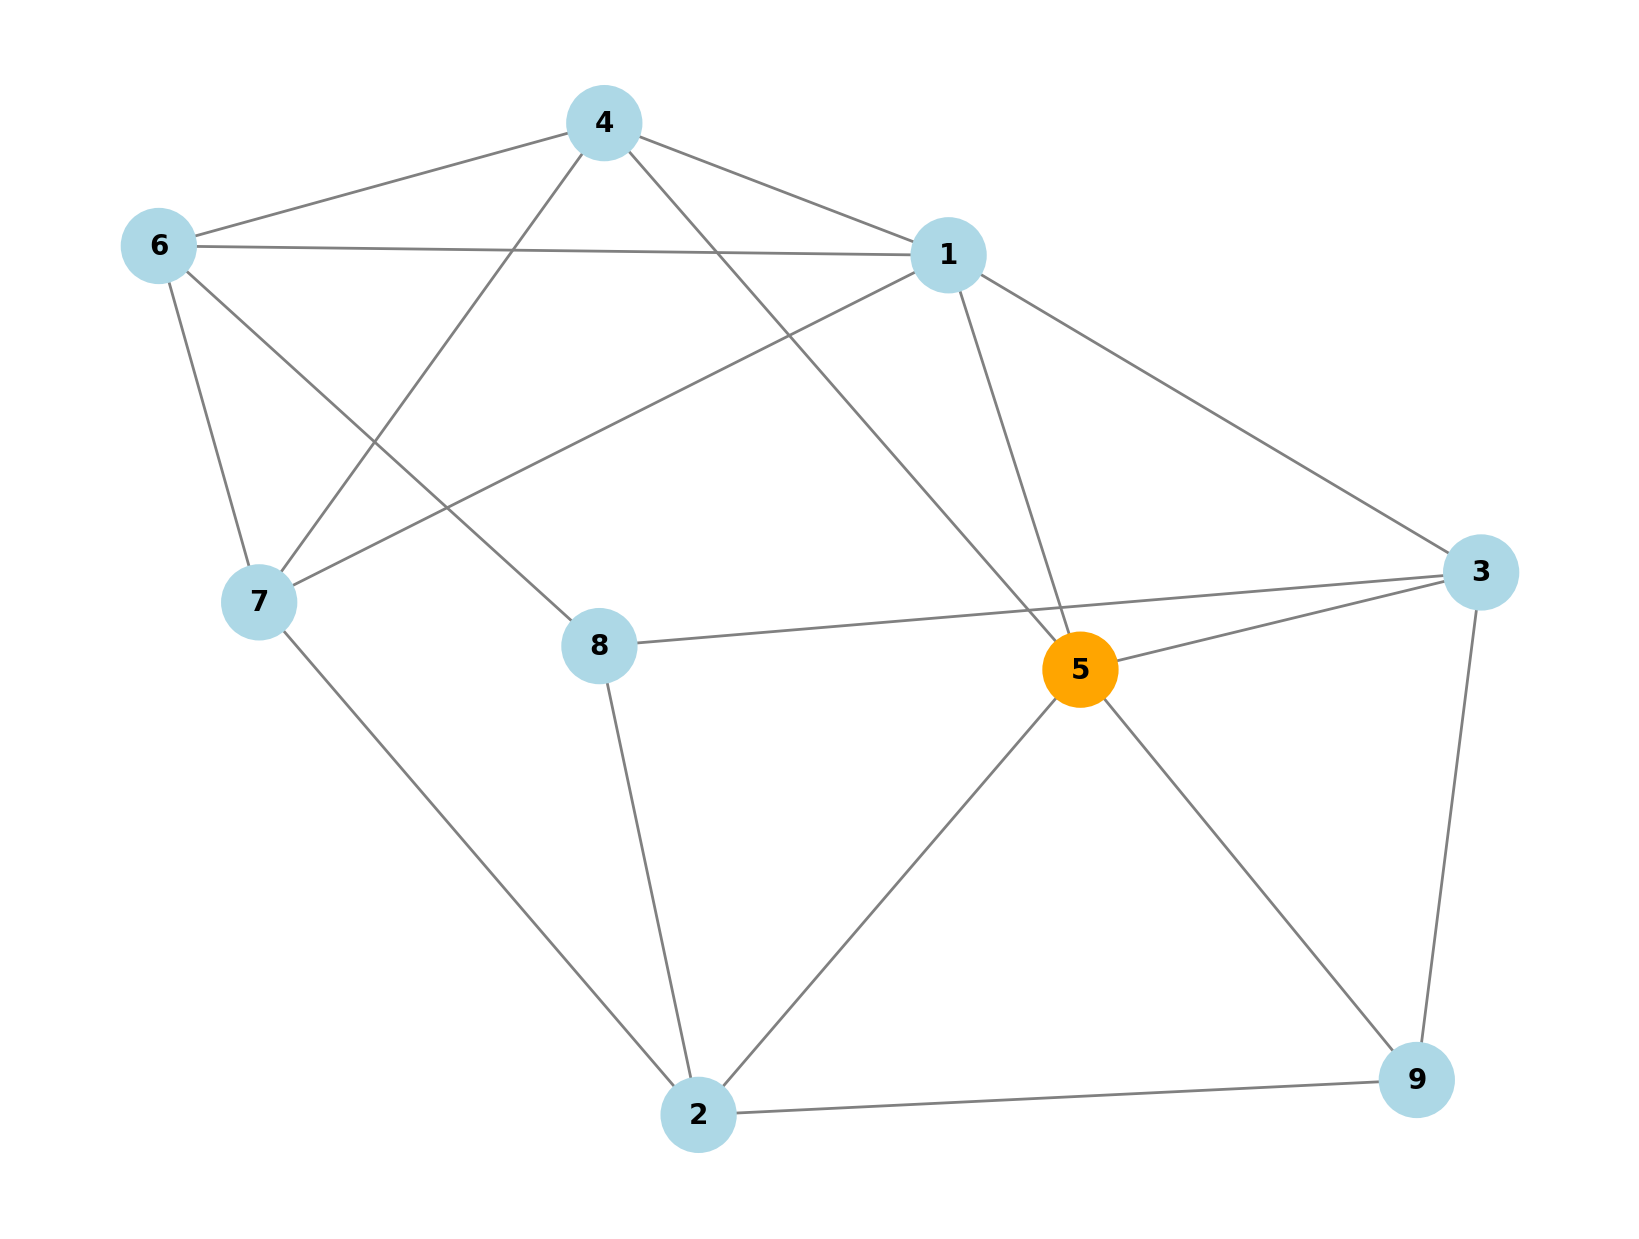
\includegraphics[width=0.4\textwidth]{images/network.png}
    \caption{Base topology network}
    \label{fig:base_network}
\end{figure}

To systematically analyze different network configurations, we defined a simple population of 10 
scenarios for the sake of clarity in this report. These scenarios explore various combinations of generation 
and storage placements within our pre-defined network. Each scenario specifies:

\begin{enumerate}
    \item The location and type of generation units (nuclear, solar, wind, or gas) at different buses
    \item The placement of storage units (Battery1 or Battery2) if any
    \item A load factor to scale the demand - in our case kept by default at 1.0 for our analysis.
\end{enumerate}

\begin{table}[H]
\centering
\begin{tabular}{l l l l}
\hline
\textbf{Scen.} & \textbf{Generation Positions} & \textbf{Storage Units} \\
\hline
\centering{1} & \{Bus 1: Nuclear, Bus 4: Solar\} & \textit{None} \\
\centering{2} & \{Bus 1: Nuclear, Bus 4: Solar\} & \{Bus 2: Bat1, Bus 7: Bat1\} \\
\centering{3} & \{Bus 1: Nuclear, Bus 4: Solar, Bus 2: Wind\} & \{Bus 7: Bat1\} \\
\centering{4} & \{Bus 2: Nuclear, Bus 4: Wind, Bus 8: Gas\} & \{Bus 1: Bat1, Bus 7: Bat2\} \\
\centering{5} & \{Bus 1: Wind, Bus 2: Solar, Bus 3: Nuclear\} & \{Bus 8: Bat1, Bus 4: Bat2\} \\
\centering{6} & \{Bus 2: Nuclear, Bus 4: Wind, Bus 7: Solar\} & \textit{None} \\
\centering{7} & \{Bus 3: Solar, Bus 4: Nuclear, Bus 8: Wind\} & \{Bus 1: Bat2\} \\
\centering{8} & \{Bus 1: Gas, Bus 4: Nuclear, Bus 7: Solar\} & \{Bus 9: Bat2, Bus 2: Bat2\} \\
\centering{9} & \{Bus 2: Wind, Bus 4: Nuclear, Bus 7: Solar, Bus 1: Solar\} & \textit{None} \\
\centering{10} & \{Bus 2: Wind, Bus 4: Nuclear, Bus 7: Solar, Bus 1: Solar\} & \{Bus 3: Bat2, Bus 9: Bat2\} \\
\hline
\end{tabular}
\caption{10 scenarios case-study from \texttt{scenarios\_parameters.csv}}
\label{tab:scenario_definitions}
\end{table}


\subsubsection{Data}
The generation units have distinct characteristics -- static limits and variable generation profiles.
Constant limits such as nuclear power plants and gas turbines have a fixed power output. Their costs and max
power were defined with dummy variables. Solar and wind are variable and depend on weather patterns hence have
a variable availability profile.

\begin{table}[h]
\centering
\begin{tabular}{l|c|c}
\hline
Type & P\textsubscript{max} (MW) & Cost (\$/MWh) \\
\hline
Nuclear & 800 & 5.0  \\
Gas & 250 & 8.0  \\
Wind & Variable & 0  \\
Solar & Variable & 0  \\
\hline
\end{tabular}
\caption{Generation Unit Specifications}
\label{tab:gen_specs}
\end{table}

\begin{table}[h]
\centering
\begin{tabular}{l|c|c|c}
\hline
Type & Power (MW) & Capacity (MWh) & Efficiency \\
\hline
Battery1 & $\pm$30 & 60 & 99\% \\
Battery2 & $\pm$55 & 110 & 99\% \\
\hline
\end{tabular}
\caption{Storage Unit Specifications}
\label{tab:storage_specs}
\end{table}


The load who can be interpreted as the demand of a little town (max. 100MW) also is variable. This hourly
fluctuating data was obtained from different sources : 
\begin{itemize}
    \item The load profile was provided by the supervising professor. An STL decomposition was applied 
    to confirm the recurring weekly patterns and seasonalities.
    \item The renewable generation data was obtained 
    from renewables.ninja \cite{renewables_ninja} for a location in Sion, Switzerland (46.231°N, 7.359°E).
    Both solar PV and wind configurations were then processed and scaled.
\end{itemize}

Their profiles can be observed below in their respective seasonal weeks. As discussed in 
Section~\ref{sec:data_preprocessing}, these week choices were made based on the mean load demand per week in 
their respective season. We aimed for the residuals to be normally distributed in these chosen weeks.

\begin{figure}[h]
  \centering
  \begin{subfigure}[b]{0.32\linewidth}
     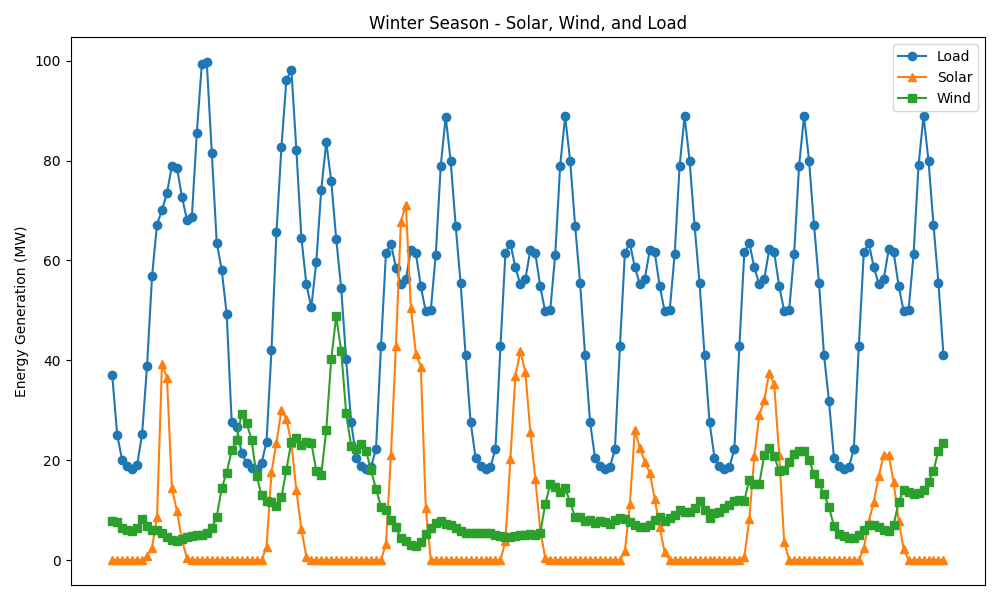
\includegraphics[width=0.8\linewidth]{images/winter_season_plot.png}
     
     \caption{Winter (WK 02)}
     \label{fig:winter_season}
  \end{subfigure}
  \hfill
  \begin{subfigure}[b]{0.32\linewidth}
     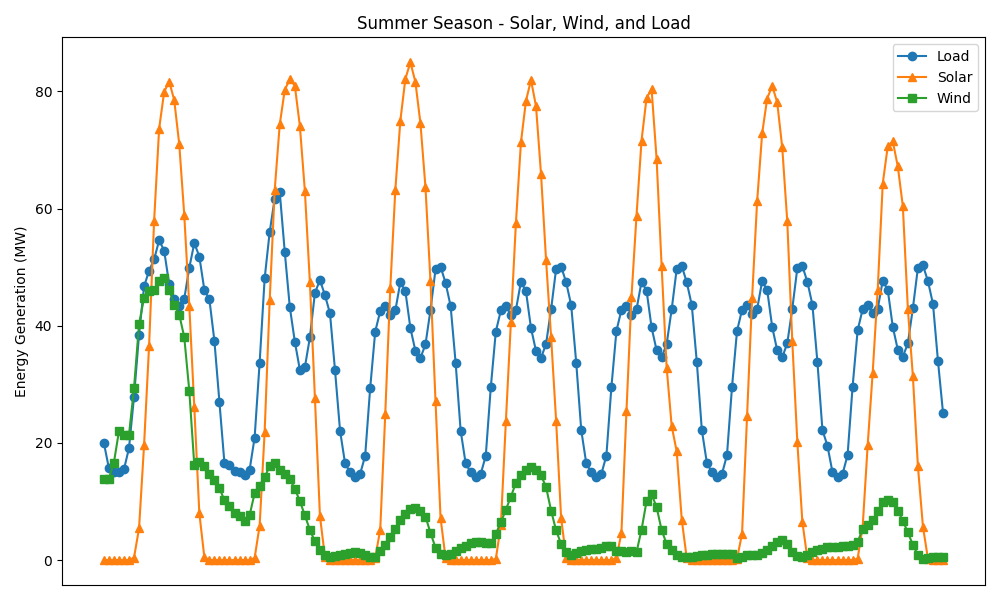
\includegraphics[width=0.8\linewidth]{images/summer_season_plot.png}
     \caption{Summer (WK 31)}
     \label{fig:summer_season}
  \end{subfigure}
  \hfill
  \begin{subfigure}[b]{0.32\linewidth}
     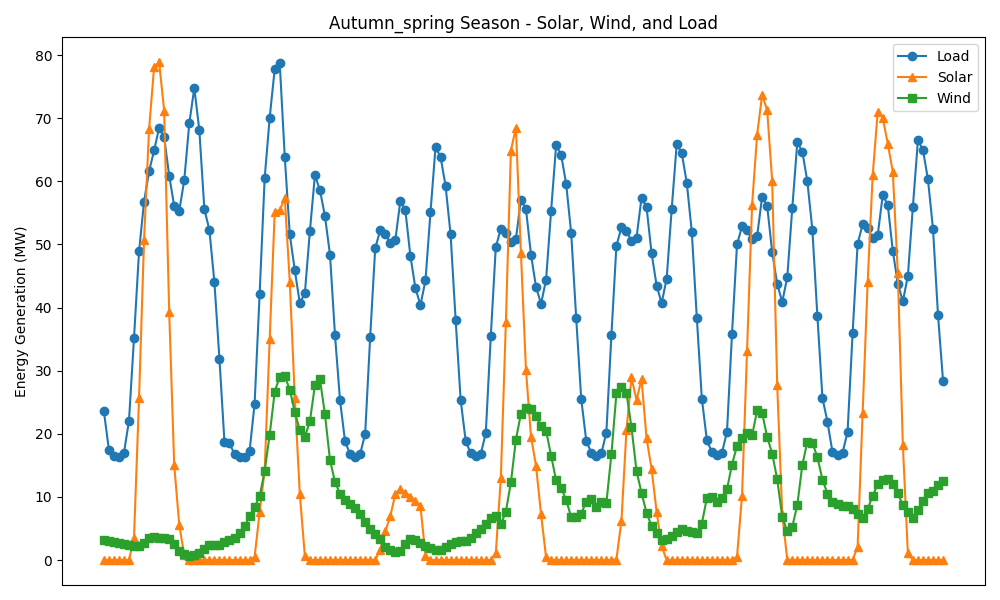
\includegraphics[width=0.8\linewidth]{images/autumn_spring_season_plot.png}
     \caption{Spring/Autumn (WK 43)}
     \label{fig:autumn_spring_season}
  \end{subfigure}
  \caption{Weekly seasonal load and generation availability profiles}
  \label{fig:weekly_seasonal_profiles}
\end{figure}


%---------------------------------------------------------------------------------------
\subsection{Operational Results}
\label{sec:operational_results}

\subsubsection{Hourly Dispatch}
Below is an example of an hourly dispatch during a summer week. As expected it shows some 24-hour seasonality in 
both the generation and demand. The stacked area plot reveals a clear daily pattern where solar generation (dashed 
orange line) peaks during midday hours while wind generation (dashed dark blue line) provides more variable output 
throughout the day. The total generation profile closely follows but slightly exceeds the demand curve (black line), 
with the excess being stored in batteries for later use.

We notice that during peak solar hours, when photovoltaic output exceeds demand, the surplus free of cost energy is 
stored in the battery. This stored energy is then discharged during evening hours when solar generation declines but 
demand remains high -- idem with the wind generation. While more difficult to notice in this configuration, the 
batteries discharge at the end of the calculation cycle to meet the condition $SOC_{0} = SOC_{final}$.

\begin{figure}[h]
    \centering
    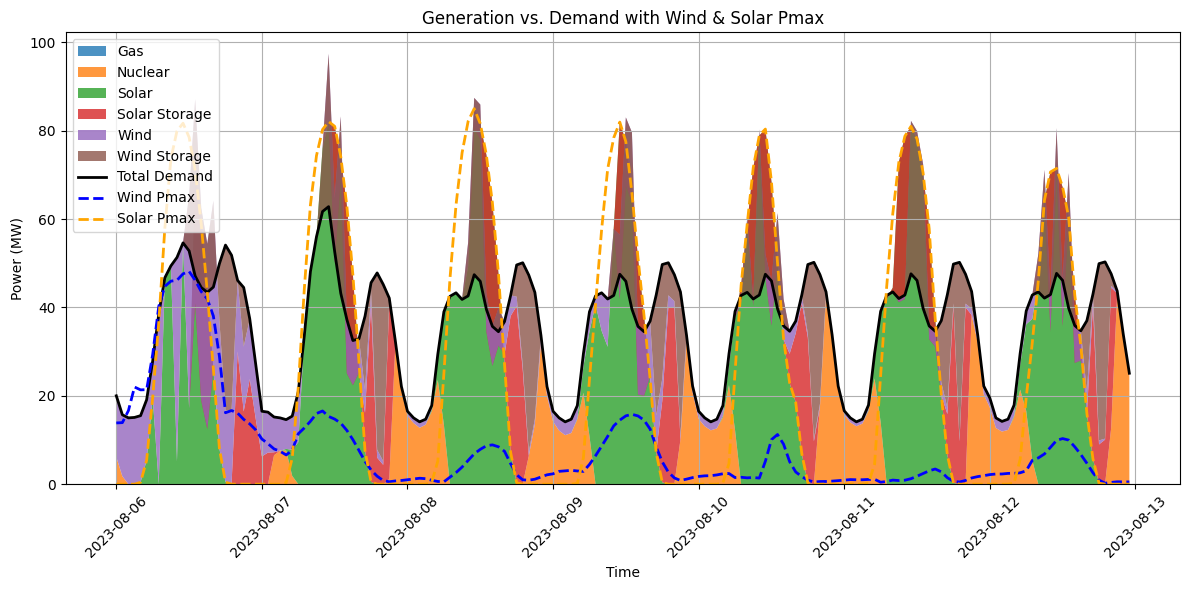
\includegraphics[width=0.8\textwidth]{images/gen_vs_demand-summer.png}
    \caption{Hourly dispatch for Scenario~5}
    \label{fig:scenario_5_dispatch}
\end{figure}

On day 2, total generation exceeds demand likely due to the battery model allowing simultaneous charging and discharging. 
Without constraints preventing concurrent charge/discharge operations, the solver can exceed single-direction power 
limits by setting both P\_charge and P\_discharge nonzero in the same hour.

\subsubsection{Feasibility \& Technical Observations}
To validate the model's behavior, particularly after simplifying from multiple loads to a single load bus, 
we analyzed the binding constraints in two contrasting scenarios (4 and 5). A review of the solver logs in 
\texttt{dcopf.py} revealed several critical binding constraints that help verify proper system operation:

\begin{figure}[h]
    \centering
    \begin{subfigure}[b]{0.48\textwidth}
        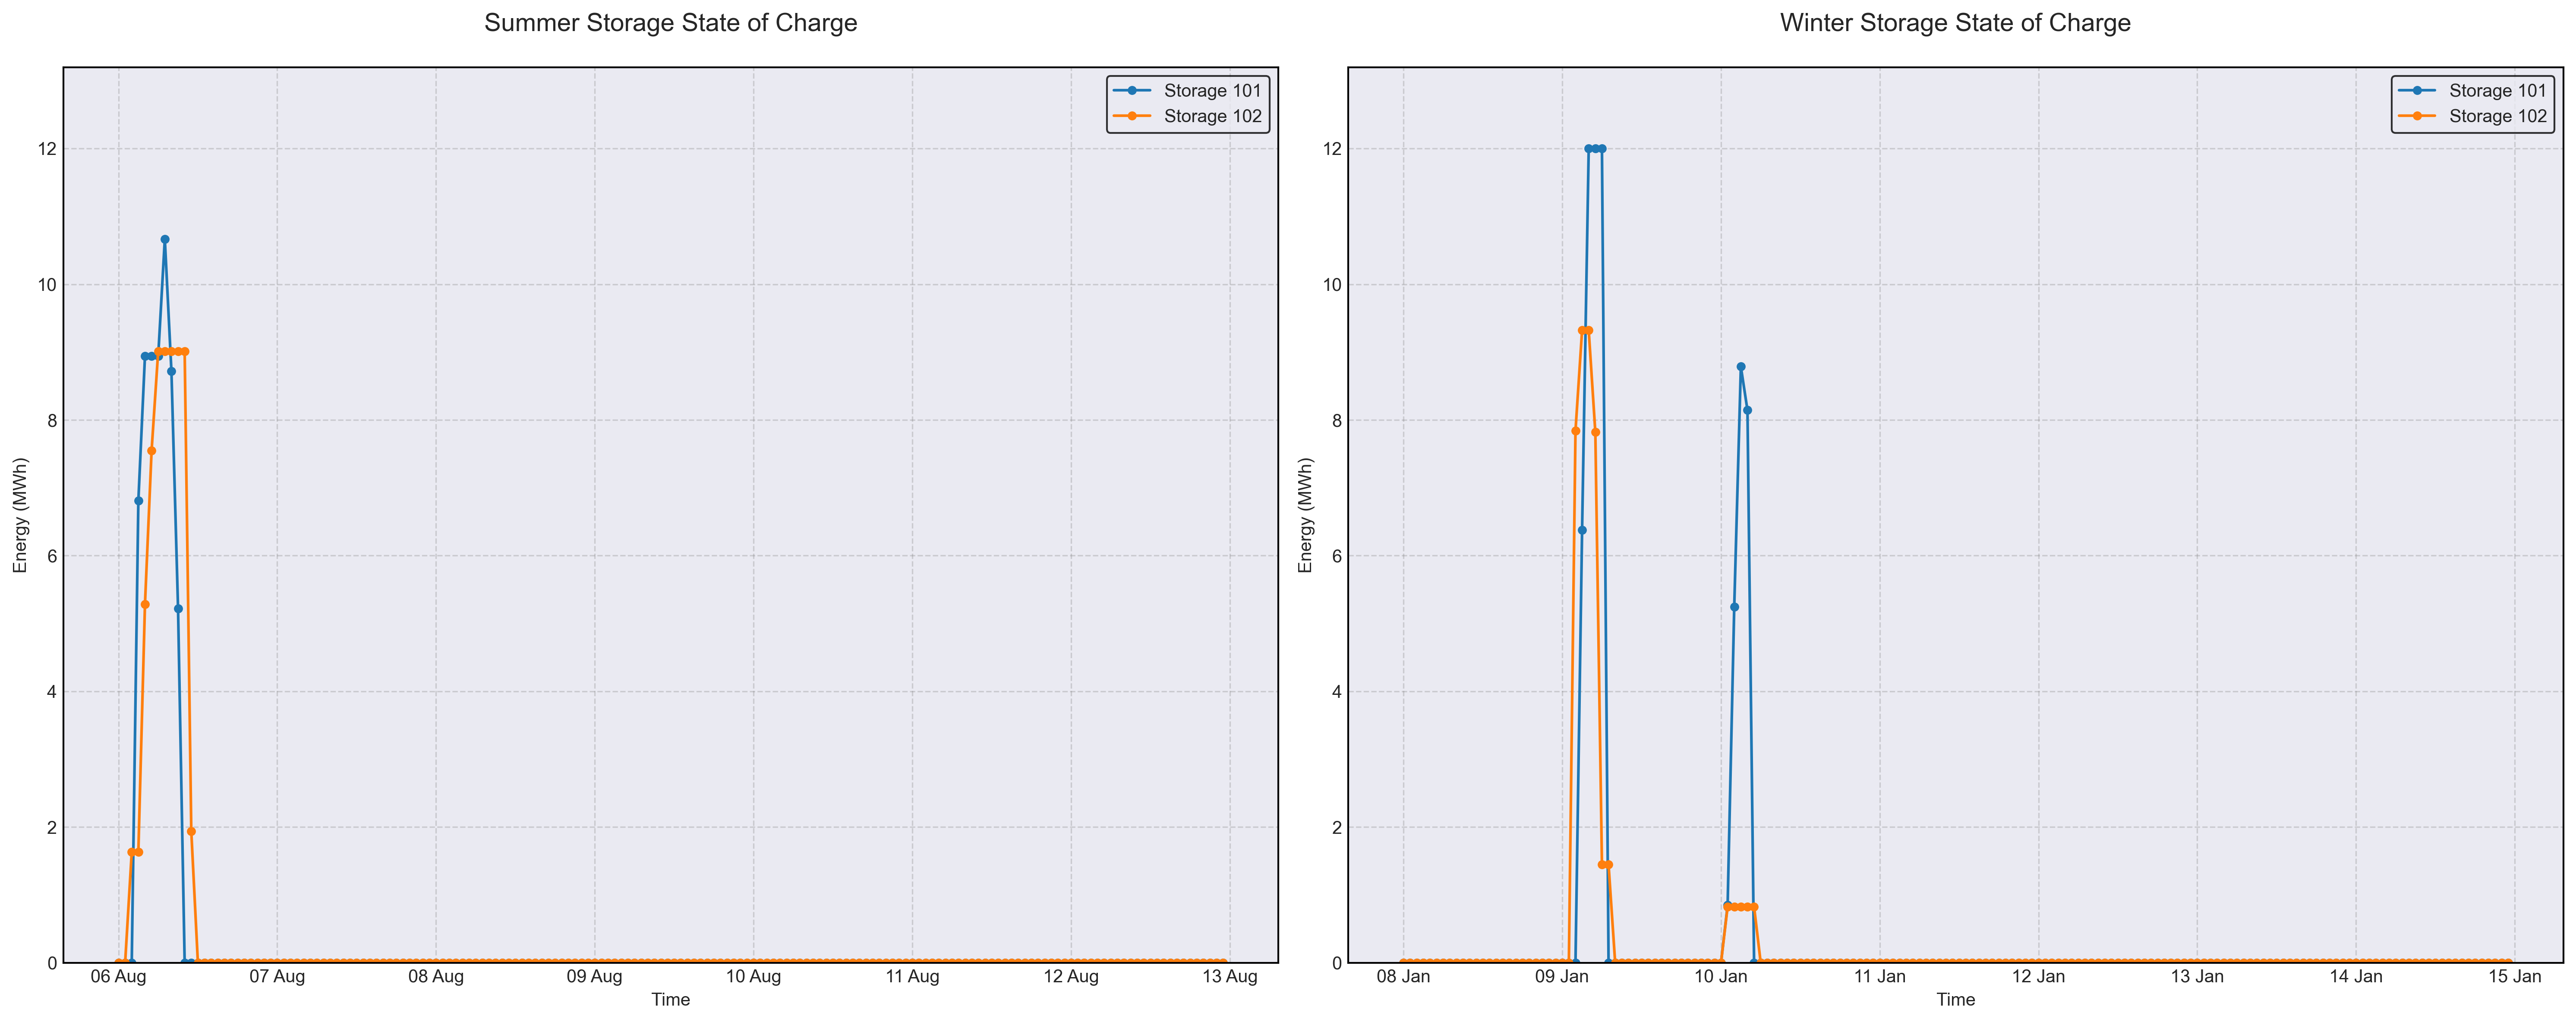
\includegraphics[width=\textwidth]{images/soc_4.png}
        \caption{Scenario~4, SoC left: Summer, right: Winter}
        \label{fig:soc_4}
    \end{subfigure}
    \hfill
    \begin{subfigure}[b]{0.48\textwidth}
        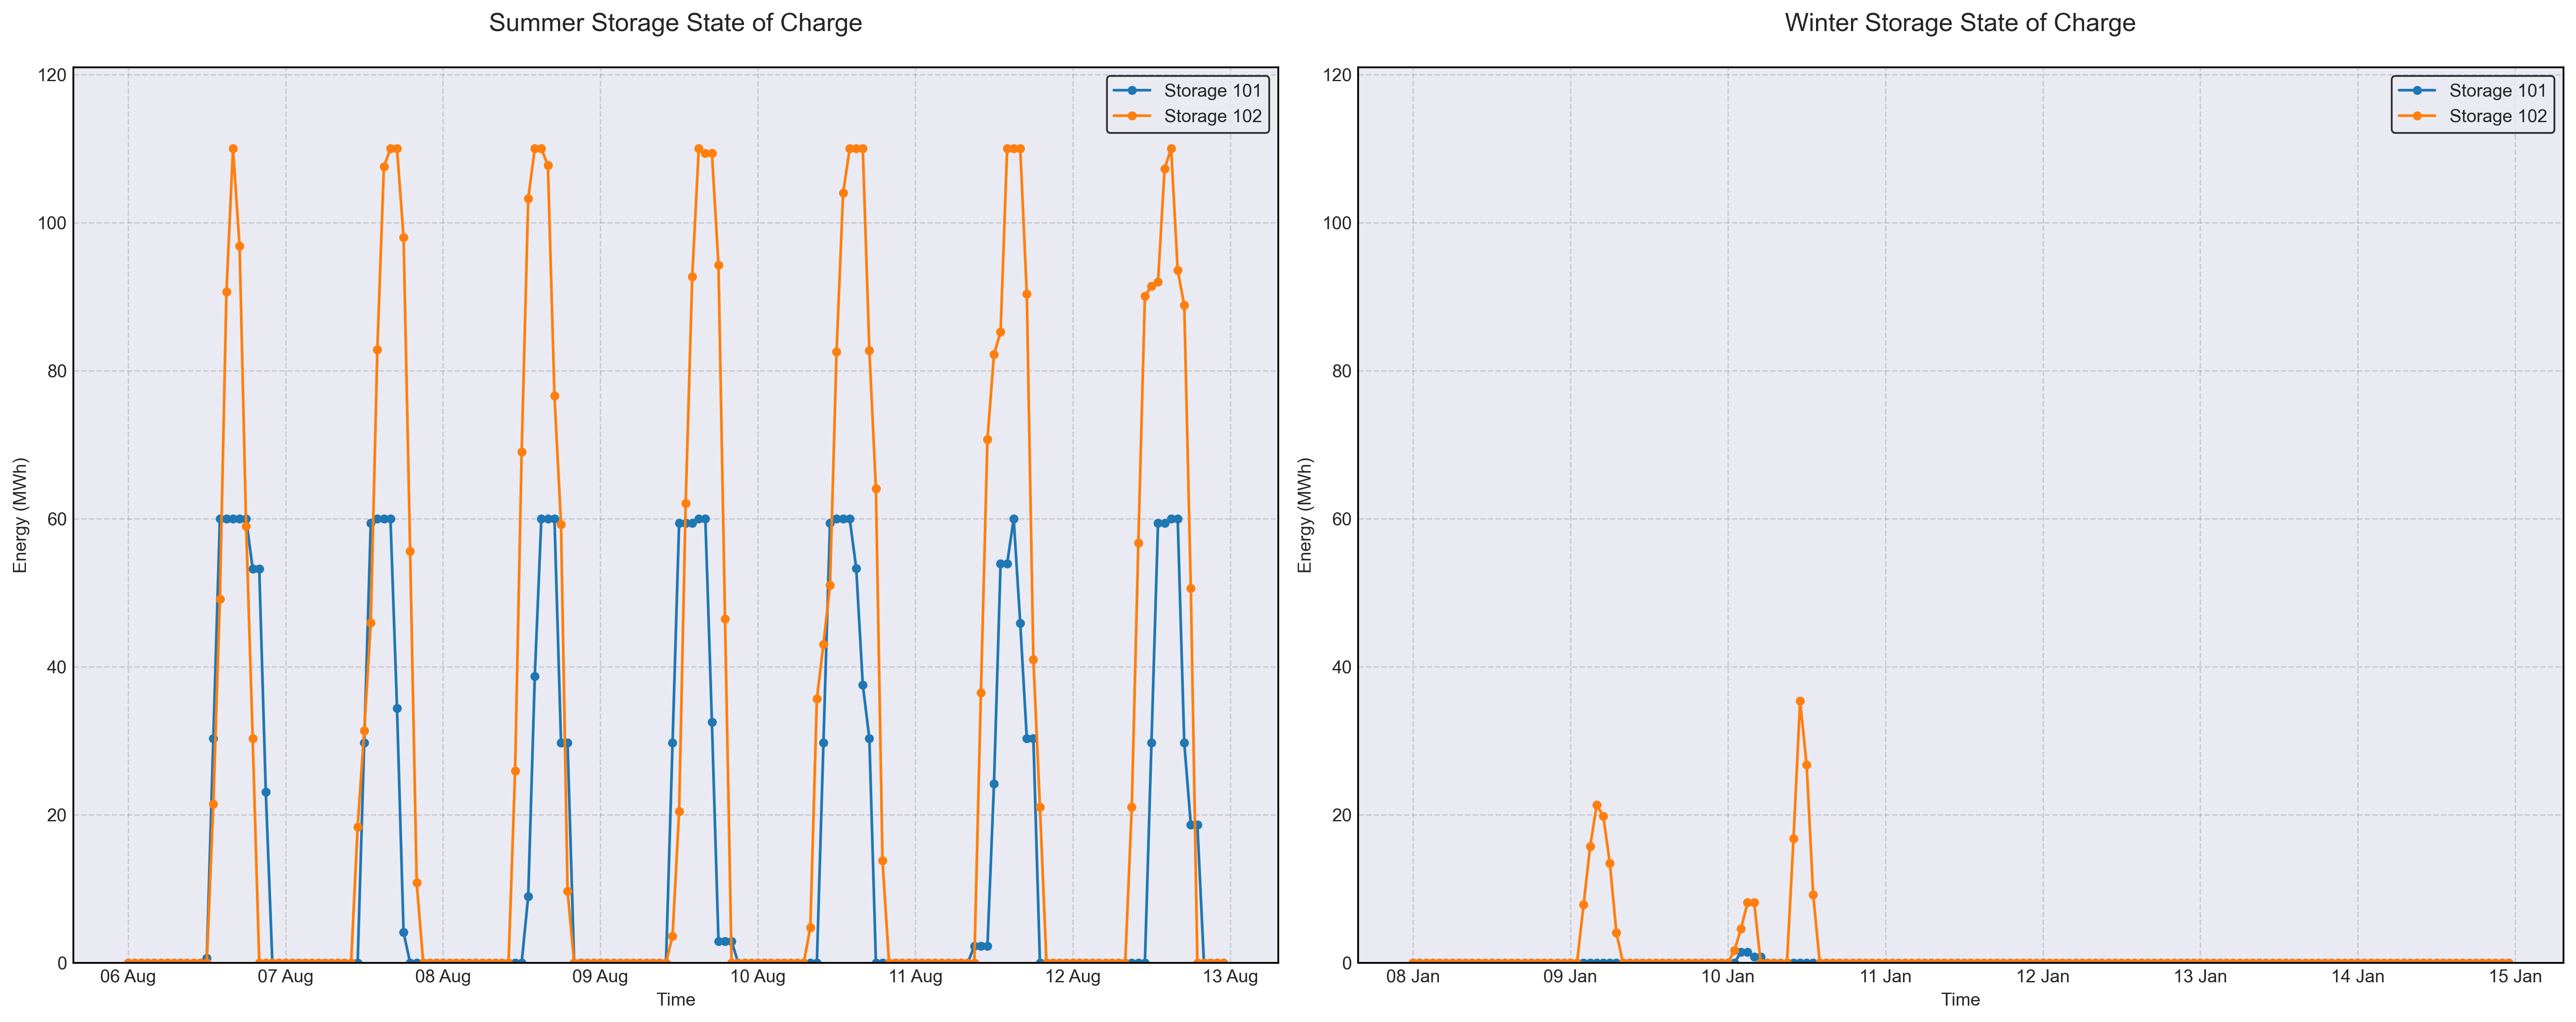
\includegraphics[width=\textwidth]{images/soc_5.png}
        \caption{Scenario~5, SoC left: Summer, right: Winter}
        \label{fig:soc_5}
    \end{subfigure}
    \caption{State of Charge comparison between Scenarios 4 and 5}
    \label{fig:soc_comparison}
\end{figure}

The State of Charge (SOC) comparison between Scenarios 4 and 5 (Fig.~\ref{fig:soc_comparison}) reveals striking 
differences in storage utilization patterns, despite both scenarios having identical generation and storage 
capacities. The key distinction lies in the generation type at Bus 2:

\begin{itemize}
    \item In Scenario 4, with nuclear generation at Bus 2, we observe relatively modest SOC variations. This 
    reflects the steady, baseload of nuclear power,(consistent output regardless of time of day). We can assume 
    that the batteries primarily serve to optimize power flow rather than accommodate large generation swings.
    They peaked on their only first usage day suggesting an emerging need for storage (60 MWh x2)
    
    \item Scenario 5, featuring solar generation at Bus 2, shows much more SoC fluctuations. The 
    pronounced midday solar peaks drive rapid battery charging-- seeing them reaching their limit every day 
    suggesting a size increase. While evening hours see significant discharge as stored energy supplements 
    the diminished solar output.On the other hand, in summer weeks the batteries are not used at all.
\end{itemize}

The network topology, particularly the lines connecting Bus 2 to buses 5, 7, 8, and 9, plays a key role in 
distributing generation and enabling storage utilization. The placement of generation units impacts power flows 
and storage patterns throughout the network.

\subsubsection{Generation dispatch}
Line flow analysis during peak hours would likely show congestion on transmission corridors connecting major generation 
sources to Bus 5. While detailed hourly patterns weren't examined, the seasonal-week models explored. In the context
of "investment" analysis, stakeholders would likely be interested in the global generation dispatch and their associated
trends.

As expected, nuclear generation increases significantly during winter periods to meet higher demand. 
Most notably in scenario 5, solar generation reaches impressive levels that even exceed nuclear output during peak 
periods, suggesting the potential for solar to serve as a primary generation source.

The annual generation profiles shown below illustrate the key seasonal patterns and generation mix across these two 
scenarios:

\begin{figure}[h]
    \centering
    \begin{subfigure}[b]{0.9\textwidth}
        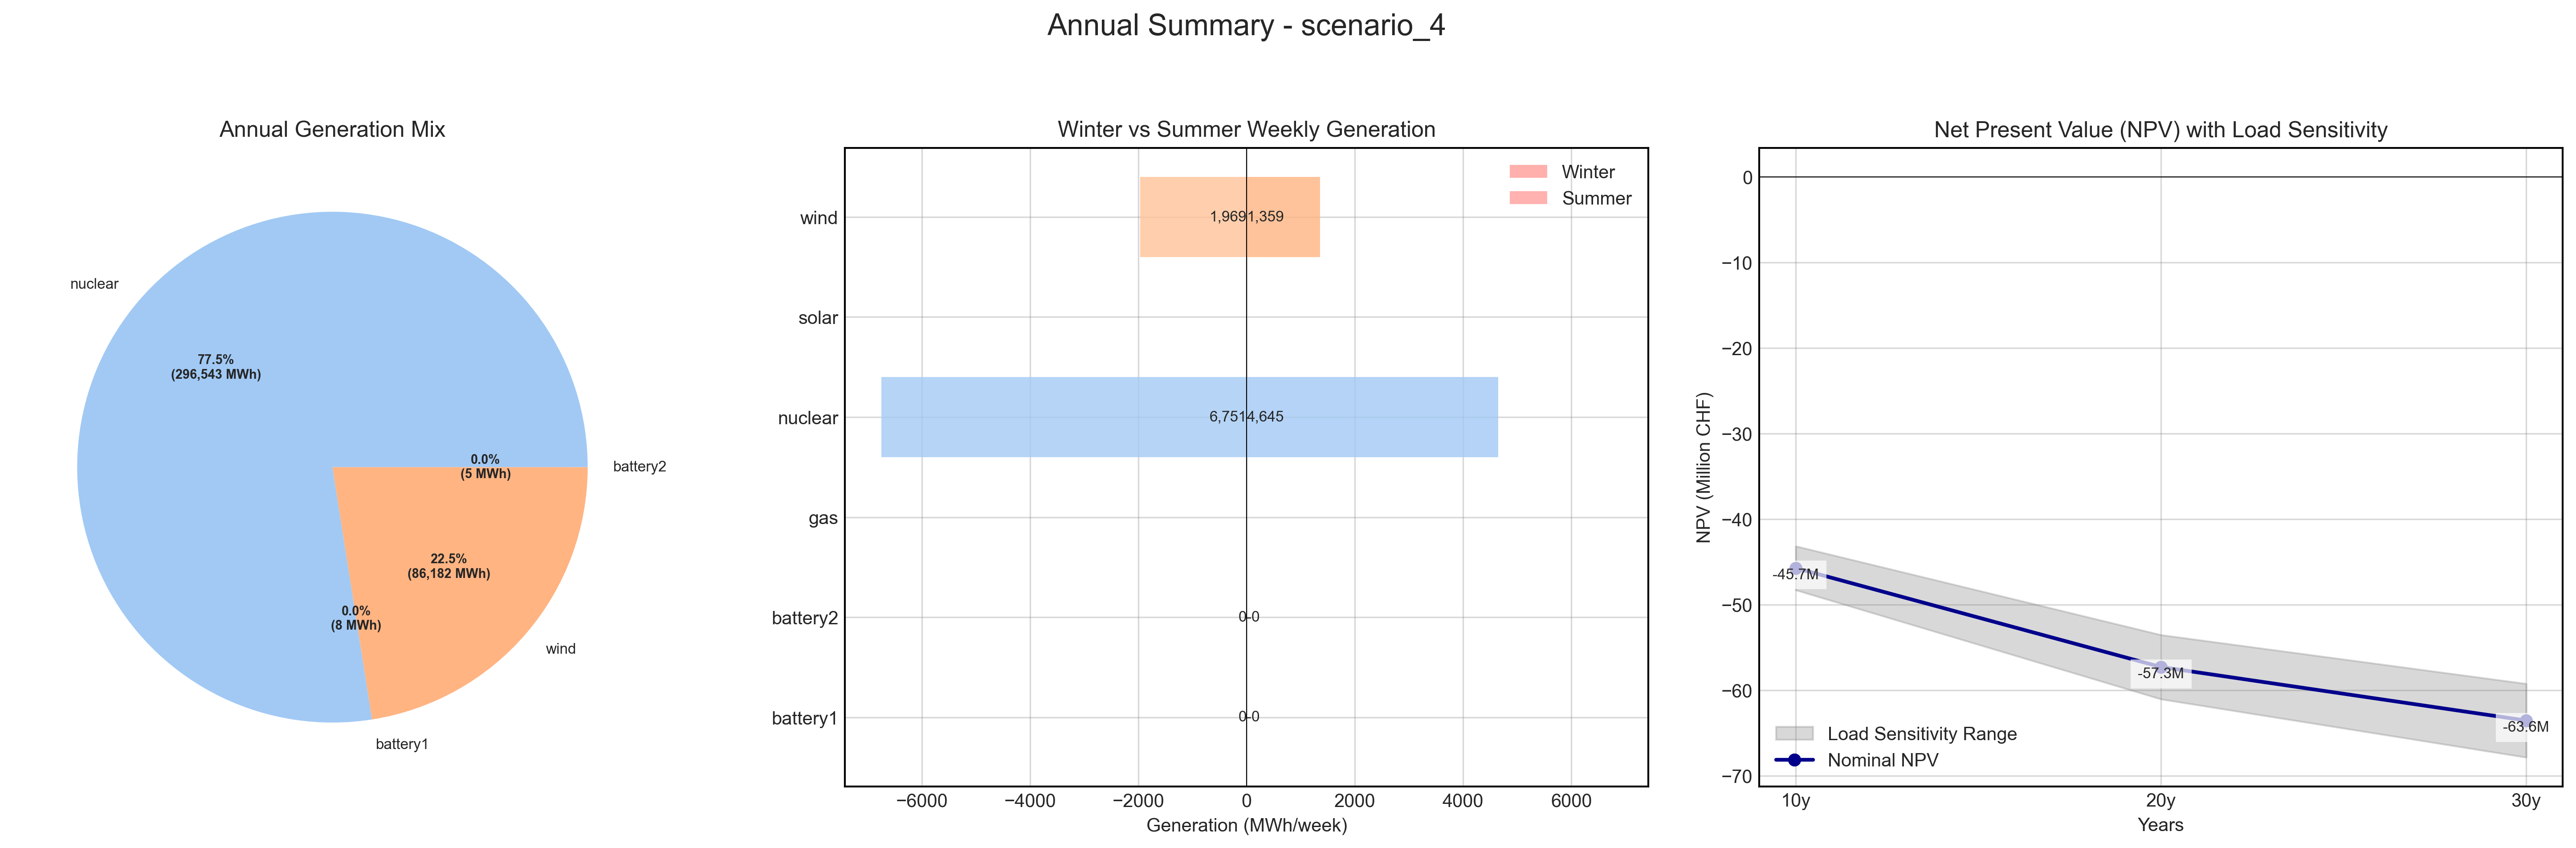
\includegraphics[width=\textwidth]{images/annual_4.png}
        % \caption{Scenario~4}
        \label{fig:annual_4}
    \end{subfigure}
    \\[\baselineskip]
    \begin{subfigure}[b]{0.9\textwidth}
        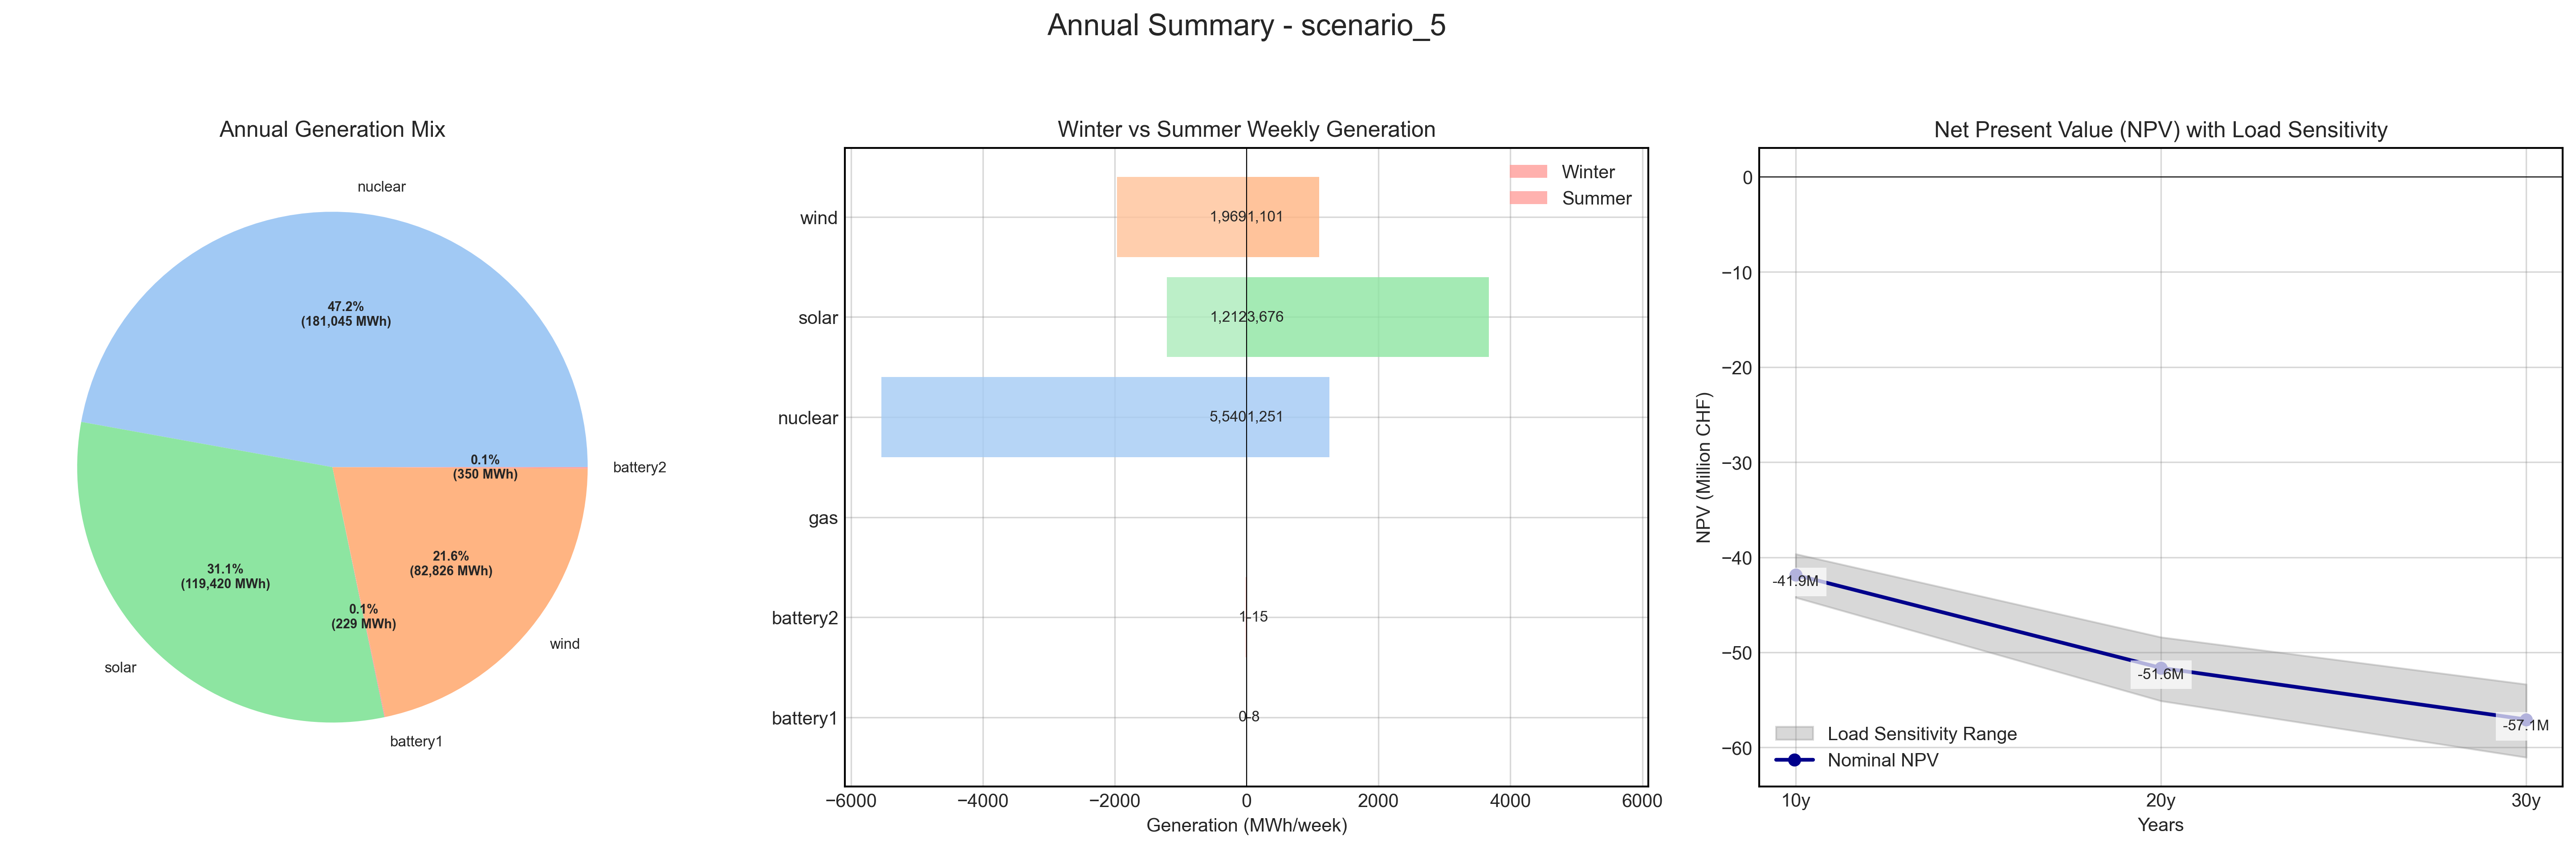
\includegraphics[width=\textwidth]{images/annual_5.png}
        %\caption{b) Scenario~5}
        \label{fig:annual_5}
    \end{subfigure}
    \caption{Summary plots of annual generation profiles for investment reports}
    \label{fig:annual_comparison}
\end{figure}

In Scenario 5, solar generation reaches impressive levels that even exceed nuclear output during peak 
periods. This scenario demonstrates how zero-cost renewable generation can create significant economic advantages.
Scenario 5 ranks second-best in overall costs whereas Scenario 4's conventional generation mix shows the worst 
cost performance, highlighting the financial benefits of integrating renewable resources into the power system.

\subsection{Investment \& Economic Analysis}
\label{sec:investment_econ}

The economic assessment focuses exclusively on renewable energy and storage assets, as these represent the key investment 
decisions. While nuclear and gas generation costs are modeled in the optimization to determine optimal dispatch, they are 
excluded from the investment analysis since our primary goal is to evaluate the financial viability of green infrastructure 
additions to an existing conventional generation fleet.

The following parameters were used: 
 \begin{table}[h]
    \centering
    \begin{tabular}{l l r}
    \hline
    \textbf{Parameter Type} & \textbf{Technology} & \textbf{Value}  \\
    \hline
    \multirow{4}{*}{CAPEX (CHF/MW)} 
        & Wind & 1'400'000 \\
        & Solar & 900'000 \\
        & Battery Type 1 & 250'000 \\
        & Battery Type 2 & 450'000 \\
    \hline
    \multirow{4}{*}{Technical Lifetime (years)}
        & Wind & 19 \\
        & Solar & 25 \\
        & Battery Type 1 & 6 \\
        & Battery Type 2 & 8 \\
    \hline
    \multirow{4}{*}{Annual OPEX (\% of CAPEX)}
        & Wind & 4\% \\
        & Solar & 2\% \\
        & Battery Type 1 & 3\% \\
        & Battery Type 2 & 4\% \\
    \hline
    \end{tabular}
    \caption{Updated financial and technical parameters used in the analysis}
    \label{tab:updated_parameters}
    \end{table}

The results illustrate a versatile platform that integrates various generation and storage technologies,
each contributing unique cost and performance profiles. Renewable assets like wind and solar offer 
attractive CAPEX values, while their associated OPEX and technical lifetimes shape long-term economics,
particularly when combined with battery systems that require more frequent replacement.

Among the scenarios analyzed, the mix in Scenario 7, which includes solar, nuclear, and wind generation 
with a single Battery Type 2, delivers the lowest annualized cost and most favorable net present values
over 10 and 30 years. This example highlights the potential of combining diverse assets to achieve a 
balanced and economically sustainable energy mix.
    
Conversely, the configuration in Scenario 4, featuring nuclear, wind, and gas with two types of battery
storage, demonstrates how additional storage and more complex asset mixes can elevate both upfront and 
recurring costs. This underlines the importance of optimizing asset selection and mix based on specific
case study requirements.
    
Overall, these results serve as a foundational example, showcasing the platform's capability to compare
different asset combinations. The insights gained here can be further refined for tailored applications
in specific case studies, emphasizing the critical role of both capital investment and long-term 
operational considerations in energy system planning.

\begin{table}[h]
\centering
\begin{tabular}{l r r r r r}
\hline
\textbf{Scen.} & \textbf{Initial Inv.} & \textbf{Annual Cost} & \textbf{10y NPV} & \textbf{30y NPV} & \textbf{Annuity} \\
\hline
7 &  2'750'000 &  942'766 &  -9'918'474 &  -15'233'659 &  1'353'167 \\
3 &  2'550'000 &  980'376 &  -9'821'150 &  -15'258'653 &  1'355'387 \\
6 &  2'300'000 &  1'048'043 &  -9'829'002 &  -15'353'770 &  1'363'836 \\
5 &  3'000'000 &  905'287 &  -10'113'189 &  -15'478'398 &  1'374'906 \\
9 &  3'200'000 &  1'048'043 &  -10'849'783 &  -16'578'091 &  1'472'589 \\
1 &  900'000 &  1'380'923 &  -10'286'888 &  -16'770'455 &  1'489'676 \\
10 &  4'100'000 &  887'122 &  -11'361'773 &  -16'896'633 &  1'500'885 \\
2 &  1'400'000 &  1'300'109 &  -10'637'014 &  -17'193'991 &  1'527'298 \\
8 &  1'800'000 &  1'275'673 &  -11'172'440 &  -17'715'738 &  1'573'644 \\
4 &  2'100'000 &  1'482'721 &  -12'967'033 &  -20'754'695 &  1'843'586 \\
\hline
\end{tabular}
\caption{Ranked by annuity, financial comparison across scenarios}
\label{tab:financial_comparison}
\end{table}


%---------------------------------------------------------------------------------------
\subsubsection{Sensitivity Analysis}

We evaluated how a \(\pm20\%\) variation in load affects each scenario's NPV over time. 
The table shows that scenarios with high gas dependency (e.g., Scenario 4) exhibit greater NPV 
volatility compared to renewable-heavy configurations. A 20\% load increase causes Scenario 4's 30-year NPV to deteriorate 
by 58\%, while Scenario 5's more diverse mix limits the impact to 75\%:

\begin{table}[ht]
\centering
\caption{NPV Analysis for Scenarios 4--5 under Load Variations (10, 20, 30-year horizons)}
\label{tab:npv_sensitivity}
\begin{tabular}{lccccc}
\hline
\textbf{Scenario} & \textbf{Load Factor} & \textbf{NPV (10yr)} & \textbf{NPV (20yr)} & \textbf{NPV (30yr)} \\
\hline
Scenario 4 & 0.8 & -11'172'440 & -15'548'394 & -17'715'738 \\
           & 1.0 & -12'967'033 & -18'400'575 & -20'754'695 \\
           & 1.2 & -14'761'626 & -21'252'756 & -23'793'652 \\
\hline
Scenario 5 & 0.8 & -8'090'551 & -11'046'381 & -12'382'718 \\
           & 1.0 & -10'113'189 & -13'807'976 & -15'478'398 \\
           & 1.2 & -12'135'827 & -16'569'571 & -18'574'078 \\
\hline
\end{tabular}
\end{table}

We can conclude that the sensitivity analysis provides insights into resilience of the scenarios.


%---------------------------------------------------------------------------------------
\subsection{Report Generation and Insights}
The AI report generates a summary of the results of individuals scenarios focus on three aspects for the individual 
scenario : 
\begin{itemize}
  \item Economic Efficiency of the Generation Mix
  \item System Composition Strengths/Weaknesses
  \item Key Recommendations for Improvement
\end{itemize}

while the global report provides a comprehensive overview of all scenarios, highlighting the 
optimal and suboptimal scenarios. It focus on the following aspects : 
\begin{itemize}
  \item Overall Trends in Cost Effectiveness
  \item Trade-offs Between Different Generation Mixes
  \item Key Success Factors in Better Performing Scenarios
  \item Recommendations for Future Scenario Design
\end{itemize}

In the individual report, while the AI effectively identifies scenarios and references analytical data, its descriptions 
remain somewhat generic and lack the depth of expert analysis. In its current configuration, it serves as a useful complement to, 
rather than replacement for experts advice. The strength lies in providing a context-based overview that 
helps investors quickly grasp the key implications of each scenario.

Also, no specific prompt engineering was performed to optimize the handling of metrics. With a more tailored 
prompt and detailed context and objectives, such as battery dimensioning or investment thresholds, the AI could generate
more targeted and insightful reports that better serve decision-making purposes.

However, the AI's global summary report effectively identifies optimal and suboptimal scenarios while providing 
comprehensive comparisons across multiple evaluation criteria -- on a superior level than the scenario-based report. The AI 
integration proves particularly valuable in generating regression analyses and uncovering relationships between predictor 
variables, leading to meaningful insights of assets usage and their associated costs. The complete global summary 
is available in the appendix.



